\documentclass[a4paper,12pt]{article}
\usepackage[top = 2.5cm, bottom = 2.5cm, left = 2.5cm, right = 2.5cm]{geometry}
% Unfortunately, LaTeX has a hard time interpreting German Umlaute. The following two lines and packages should help. If it doesn't work for you please let me know.
\usepackage[T1]{fontenc}
\usepackage[utf8]{inputenc}
% The following two packages - multirow and booktabs - are needed to create nice looking tables.
\usepackage{multirow} % Multirow is for tables with multiple rows within one cell.
\usepackage{booktabs} % For even nicer tables.
% As we usually want to include some plots (.pdf files) we need a package for that.
\usepackage{graphicx}
\usepackage{tikz}
% The default setting of LaTeX is to indent new paragraphs. This is useful for articles. But not really nice for homework problem sets. The following command sets the indent to 0.
\usepackage[spanish]{babel}
\usepackage{setspace}
\setlength{\parindent}{0in}
% Package to place figures where you want them.
\usepackage{float}
% The fancyhdr package let's us create nice headers.
\usepackage{fancyhdr}
\usepackage{amsmath}
\usepackage{amssymb}
\usepackage{natbib}
\usepackage{apalike}
\usepackage{graphicx}
\usepackage{subcaption}
\usepackage{booktabs}
\usepackage{etoolbox}
\usepackage{amsthm}
\AtBeginEnvironment{align}{\setcounter{equation}{0}}
\newenvironment{solution}
  {\renewcommand\qedsymbol{$\blacksquare$}\begin{proof}[Solución]}
  {\end{proof}}
\pagestyle{fancy}

\fancyhf{}

\lhead{\footnotesize Tarea 3}
\rhead{\footnotesize  Rompich}
\cfoot{\footnotesize \thepage}



\begin{document}
    \thispagestyle{empty} % This command disables the header on the first page.

    \begin{tabular}{p{15.5cm}} % This is a simple tabular environment to align your text nicely
    \begin{tabbing}
    Universidad del Valle de Guatemala 
    \\
    Departamento de Matemática\\ Licenciatura en Matemática Aplicada \\ Fecha de entrega: 18 de marzo de 2021  \\
    Rudik R. Rompich   - Carné: 19857\\
    \end{tabbing}
    Estadística 2 - Eugenio Aristondo \\
    \hline % \hline produces horizontal lines.
    \\
    \end{tabular} % Our tabular environment ends here.
    \vspace*{0.3cm} % Now we want to add some vertical space in between the line and our title.
    \begin{center} % Everything within the center environment is centered.
    {\Large \bf HDT 3
} % <---- Don't forget to put in the right number
        \vspace{2mm}
    \end{center}
    \vspace{0.4cm}
Se  realizó un  experimento para  investigar  el  efecto  de  la  capacitación gerencial  sobre  la habilidad de los supervisores para tomar decisiones en una gran compañía. Se seleccionaron 16  supervisores  y  ocho  fueron  escogidos  al  azar  para recibir  capacitación  administrativa. Cuatro  supervisores capacitados  y  cuatro  no capacitados  se  seleccionaron al  azar  para funcionar  en  una  situación  en  la  que  surgió un  problema  común.  A  los  otros  ocho supervisores  se les  presentó  una  situación  de  emergencia  en  la  que  los procedimientos estándar  no  podían  usarse.  La  respuesta fue  una  clasificación  de  conducta  administrativa para cada supervisor, evaluada al calificar un esquema diseñado por el experimentador.

\begin{center}
    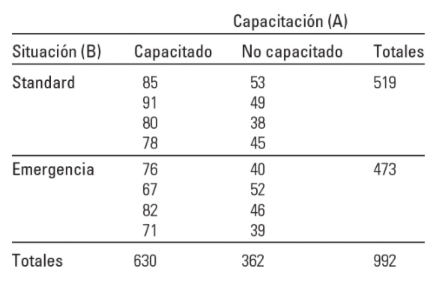
\includegraphics[scale=0.8]{Imagenes/tabla.png}
\end{center}
\begin{enumerate}
    
\item ¿Cuáles son las unidades experimentales de este experimento?
\begin{solution}
Las unidades experimentales hacen referencia a los supervisores. 
\end{solution}
\item  ¿Cuáles son los dos factores considerados en el experimento?
\begin{solution}
Los factores hacen referencia a los supervisores Capacitados y No capacitados.
\end{solution}
\item ¿Cuáles son los niveles de cada factor?
\begin{solution}
Situación estándar y situación de emergencia.
\end{solution}
\item ¿Cuántos tratamientos hay en el experimento?\begin{solution}
Hay 2 tratamientos. 
\end{solution}
\item ¿Qué tipo de diseño experimental se ha empleado?
\begin{solution}
Es un experimento de efectos aleatorios, ya que se enfocará en analizar conjuntamente las diferencias entre Capacitados-No capacitados con Estándar-Emergencia. Además, es un experimento balanceado ya que todos los niveles y tratamientos tienen la misma cantidad de datos. Es un diseño de comparación.
\end{solution}

\item Construya la tabla ANOVA para este experimento.
\begin{center}
    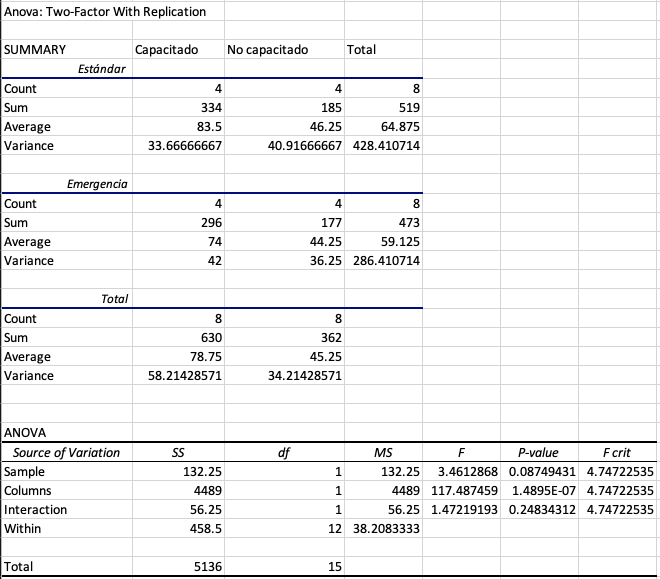
\includegraphics[scale=0.5]{Imagenes/lol.png}
\end{center}
\item ¿Hay una interacción significativa entre la presencia o ausencia de capacitación y el tipo de situación de toma de decisiones? Pruebe al nivel de 5\% de significancia.
\begin{solution}
Por la prueba $F_\alpha$. En donde $F>F_\alpha$, se puede afirmar que hay evidencia significativa para afirmar que sí una interacción significativa entre capacitados y no capacitados; y sus respectivas interacciones con la toma de decisiones. La diferencia es bastante alta. 
\end{solution}
\item ¿Los datos indican una diferencia significativa en calificaciones de conducta para los dos tipos de situaciones al nivel de significancia de 5\%?
\begin{solution}
Por la prueba $F_\alpha$. En donde $F<F_\alpha$, hay evidencia significativa para afirmar que no existe una diferencia significativa entre los dos tipos de situaciones.
\end{solution}
\item ¿Las  calificaciones  de  conducta  difieren significativamente  para  los  dos  tipos  de categorías de capacitación al nivel de significancia de 5\%?
\begin{solution}
Por la prueba $F_\alpha$. En donde $F<F_\alpha$, hay evidencia significativa para afirmar que los dos tipos de categorías de capacitación no difieren significativamente.
\end{solution}
\end{enumerate}

\end{document}